
\begin{titlepage}
    % Strona tytułowa
    \vbox to\textheight{\hyphenpenalty=10000
    \begin{center}
	\begin{tabular}{p{107mm} p{9cm}}
	    \begin{minipage}{9cm}
	      \begin{center}
	      Politechnika Warszawska \\
	      Wydział Elektroniki i~Technik Informacyjnych \\
	      Instytut Informatyki
	      \end{center}
	    \end{minipage}
	    &
	    \begin{minipage}{8cm}
	    \begin{flushleft}
	     \footnotesize
	      Rok akademicki 2012/2013
	    \vspace*{2.75\baselineskip}
	    \end{flushleft}
	    \end{minipage} \\
	\end{tabular}
	\vspace*{3.75\baselineskip}
	\par\vspace{\smallskipamount}
	\vspace*{2\baselineskip}{\LARGE Praca dyplomowa inżynierska\par}
	\vspace{3\baselineskip}{\LARGE\strut Andrzej Fiedukowicz\par}
	\vspace*{2\baselineskip}{\huge\bfseries Implementacja symulatora ruchu obiektów w środowisku miejskim na potrzeby systemu fuzji danych
	\par}

	\vspace*{7\baselineskip}
	\hfill\mbox{}\par\vspace*{\baselineskip}\noindent
	\begin{tabular}[b]{@{}p{3cm}@{\ }l@{}}
	    {\large\hfill } & {\large }
	\end{tabular}
	\hfill
	\begin{tabular}[b]{@{}l@{}}
	Opiekun pracy: \\[\smallskipamount]
	{\large dr inż. Rafał Biedrzycki}
	\end{tabular}\par
	\vspace*{4\baselineskip}
    \begin{tabular}{p{\textwidth}}
    \begin{flushleft}
	\begin{minipage}{7cm}
	Ocena \dotfill
	\par\vspace{1.6\baselineskip}
	\dotfill
	\par\noindent
	\centerline{\footnotesize Podpis Przewodniczącego} \par
	\centerline{\footnotesize Komisji Egzaminu Dyplomowego}\par
	\end{minipage}
    \end{flushleft}
    \end{tabular}
    \end{center}}

    % Życiorys
    \newpage\thispagestyle{empty}
    \begin{tabular}{p{5cm} p{12cm}}
    \begin{minipage}{5cm}
    \center
    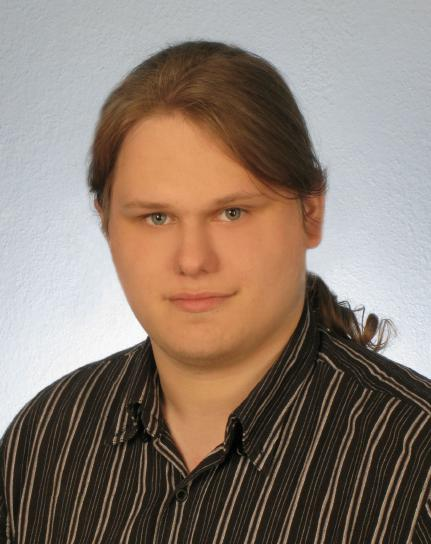
\includegraphics[height=5.8cm,width=4.5cm]{img/foto.jpg}
    \end{minipage}
    &
    \begin{minipage}{12cm}
    \begin{flushleft}
    \par\noindent\vspace{1\baselineskip}
    \begin{tabular}[h]{l l}
    {\normalsize\it Specjalność:} & Informatyka -- \\
    & Inżynieria systemów \\
    & informatycznych \\
    \end{tabular}
    \par\noindent\vspace{1\baselineskip}
    \begin{tabular}[h]{l l}
    {\normalsize\it Data urodzenia:} & {\normalsize 2 maja 1990~r.}
    \end{tabular}
    \par\noindent\vspace{1\baselineskip}
    \begin{tabular}[h]{l l}
    {\normalsize\it Data rozpoczęcia studiów:} & {\normalsize 22 luty 2010 r.}
    \end{tabular}
    \par\noindent\vspace{1\baselineskip}
    \end{flushleft}
    \end{minipage}
    \end{tabular}
    \vspace*{1\baselineskip}
    \begin{center}
	{\large\bfseries Życiorys}\par\bigskip
    \end{center}

    \indent
    Nazywam się Andrzej Fiedukowicz, urodziłem się 2 maja 1990 roku w Warszawie. W roku 2003 ukończyłem Szkołę Podstawową w Chocianowie, a w roku 2006 Gimnazjum nr 1 w Józefowie. Naukę kontynuowałem w IV Liceum Ogólnokształcącego im. Adama Mickiewicza w Warszawie, które ukończyłem zdając maturę w 2009 roku. W lutym roku 2010 rozpocząłem studia na wydziale Elektroniki i Technik Informacyjnych Politechniki Warszawskiej na kierunku Informatyka w toku studiów wybierając specjalizację Inżynieria Systemów Informatycznych. Od maja 2012 roku pracuję zawodowo jako programista języka C++.
    \par
    \vspace{2\baselineskip}
    \hfill\parbox{15em}{{\small\dotfill}\\[-.3ex]
    \centerline{\footnotesize podpis studenta}}\par
    \vspace{3\baselineskip}
    \begin{center}
 	{\large\bfseries Egzamin dyplomowy} \par\bigskip\bigskip
    \end{center}
    \par\noindent\vspace{1.5\baselineskip}
    Złożył egzamin dyplomowy w dn. \dotfill
    \par\noindent\vspace{1.5\baselineskip}
    Z wynikiem \dotfill
    \par\noindent\vspace{1.5\baselineskip}
    Ogólny wynik studiów \dotfill
    \par\noindent\vspace{1.5\baselineskip}
    Dodatkowe wnioski i uwagi Komisji \dotfill
    \par\noindent\vspace{1.5\baselineskip}
    \dotfill

    % Streszczenie
    \newpage\thispagestyle{empty}
    \vspace*{2\baselineskip}
    \begin{center}
	{\large\bfseries Streszczenie}\par\bigskip
    \end{center}

    {\itshape
    \par{
    Praca opisuje podejście do tworzenie symulatorów mających stanowić źródło danych dla systemów fuzji danych oraz wprowadza do związanej z tym problamatyki.
	}    
    \par{
	W pracy opisano również proces tworzenia modelu ruchu obiektów w środowisku miejskim. Stworzono model uwzględniający specyfikę systemów fuzji danych. Zaprezentowano podejście do tworzenia ogólnej architekutry aplikacji wykorzystującej zaproponowany model oraz wykorzystano tę architekturę by stworzyć konkretną implementację systemu symulującego zdolnego do współpracy z systemem fuzji daych.
	}
	\par{
	W ramach pracy przeprowadzono także badania wydajnościowe, które pozwoliły okreslic jakiego rodzaju ograniczenia programowo-sprzętowe są kluczowe z punktu widzenia możliwości omawianych systemów.
	}
    }
    \vspace*{1\baselineskip}

    \noindent{\bf Słowa kluczowe}: {\itshape symulator, środowiso miejskie, fuzja danych.}
    \par
    \vspace{4\baselineskip}
    \begin{center}
	{\large\bfseries Abstract}\par\bigskip
    \end{center}
    \noindent{\bf Title}: {\itshape Implementation of urban environment simulator for purposes of data fusion system.
    }\par
    \vspace*{1\baselineskip}
    {\itshape
    \par{
    This thesis describes approach to creating simulator feeding data fusion systems and introduces to problems associated with it.
	}
    \par{
    This thessis also describes process of creating movement model of objects in urban environment designed to work as part of data fusion system. Model that meets data fusion specific requirements was created. Aproach to creating general architecture of application using created model was shown together with its specific implementation capable of working with data fusion system.
	}
	\par{
	This thessis was also a base to conduct some performance benchmarks which allowed to determine which kind of software or hardware limitation is currently crucial from the described systems point of view.
	}
    }
    \vspace*{1\baselineskip}

    \noindent{\bf Key words}: {\itshape simulation, urban environment, data fusion}

\end{titlepage}

% ex: set tabstop=4 shiftwidth=4 softtabstop=4 noexpandtab fileformat=unix filetype=tex spelllang=pl,en spell:
